\documentclass[12pt]{article}
\usepackage{amsmath,amssymb,amsthm, amsfonts}
\usepackage{tikz, graphicx, subcaption, caption}
\usetikzlibrary{positioning}
\usepackage{color}

\begin{document}

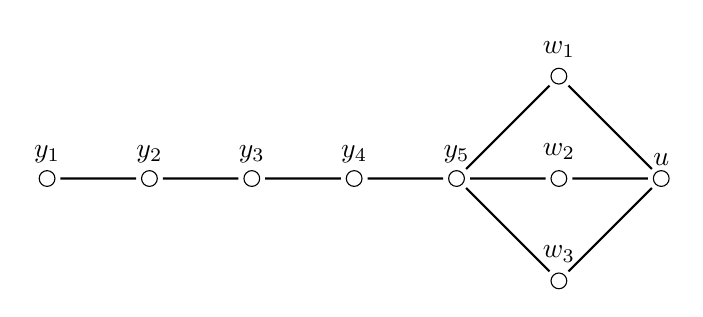
\begin{tikzpicture}[scale=1.3,every node/.style={draw,shape=circle,outer sep=2pt,inner sep=1pt,minimum size=.2cm}]		
\node[fill=none, label={[yshift=-5pt]$y_1$}]  (00) at (0,0) {};
\node[fill=none, label={[yshift=-5pt]$y_2$}]  (01) at (1,0) {};
\node[fill=none, label={[yshift=-5pt]$y_3$}]  (02) at (2,0) {};
\node[fill=none, label={[yshift=-5pt]$y_4$}]  (03) at (3,0) {};
\node[fill=none, label={[yshift=-5pt]$y_5$}]  (04) at (4,0) {};
\node[fill=none, label={[yshift=-5pt]$w_2$}]  (05) at (5,0) {};
\node[fill=none, label={[yshift=-5pt]$u$}]  (06) at (6,0) {};
\node[fill=none, label={[yshift=-5pt]$w_1$}]  (07) at (5,1) {};
\node[fill=none, label={[yshift=-5pt]$w_3$}]  (08) at (5,-1) {};
		
%Drawing the thick edges
\draw[thick] (00)--(01)--(02)--(03)--(04)--(05)--(06)--(07)--(04);
\draw[thick] (04)--(08)--(06);
\end{tikzpicture}

\end{document}